\documentclass[11pt,twoside,a4paper]{book}  
% definice dokumentu
\usepackage[english]{babel}
\usepackage[T1]{fontenc} 				% pouzije EC fonty 
\usepackage[utf8]{inputenc} 			% utf8 kódování vstupu 
\usepackage[square, numbers]{natbib}	% sazba pouzite literatury
%\usepackage{indentfirst} 				% 1. odstavec jako v cestine, pro práci v aj možno zakomentovat
\usepackage{fancyhdr}					% tisk hlaviček a patiček stránek
\usepackage{nomencl} 					% umožňuje snadno definovat zkratky a jejich seznam

%%%%%%%%%%%%%%%%%%%%%%%%%%%%%%%%%%%%%%%%%%%%%%%%%%%%%%%%%%%%%%%
% informace o práci
\newcommand\WorkTitle{Interactive visualization system for hybrid active pixel detectors within the ATLAS experiment at CERN}		% název
\newcommand\FirstandFamilyName{Petr Mánek}																							% autor
\newcommand\Supervisor{Ing. Stanislav Pospíšil, DrSc.}																				% vedoucí

\newcommand\TypeOfWork{Bachelor's Project}	% typ práce [Diplomová práce | Bakalářská práce | Bachelor's Project | Master's Thesis ]	

% Nastavte následují podle vašeho oboru a programu (pomoc hledejte na http://www.fel.cvut.cz/cz/education/bk/prehled.html)								
\newcommand\StudProgram{Open Informatics}											% program
\newcommand\StudBranch{Computer and Information Science}           					% obor

%%%%%%%%%%%%%%%%%%%%%%%%%%%%%%%%%%%%%%%%%%%%%%%%%%%%%%%%%%%%%%%
% minimální importy
\usepackage{graphicx}					% pro vkládání obrázků
\usepackage{k336_thesis_macros} 		% specialni makra pro formatovani DP a BP
\usepackage[
pdftitle={\WorkTitle},				% nastaví v informacích o pdf název
pdfauthor={\FirstandFamilyName},	% nastaví v informacích o pdf autora
colorlinks=true,					% před tiskem doporučujeme nastavit na false, aby odkazy a url nebyly šedé při ČB tisku
breaklinks=true,
urlcolor=red,
citecolor=blue,
linkcolor=blue,
unicode=true,
]
{hyperref}								% pro zobrazování "prokliknutelných" linků 

% rozšiřující importy
\usepackage{caption}			%popisy
\usepackage{subcaption}			%popisy (členité)
\usepackage[newfloat]{minted}             %lepší zdrojové kódy
\usepackage{algorithmicx} 		%slouží pro zápis algoritmů
\usepackage{algpseudocode} 		%slouží pro výpis pseudokódu
\usepackage{tikz}		        %TeX obrázky
\usetikzlibrary{trees,calc,positioning,shapes.geometric,matrix,arrows,decorations.pathreplacing,arrows.meta,decorations.markings,math}
\usepackage{inconsolata}		%hezký monospace font
\usepackage{xcolor}				%barvičky
\usepackage{pgf-umlsd}			%UML sekvence
\usepackage{tikz-timing}		%časové grafy

%%%%%%%%%%%%%%%%%%%%%%%%%%%%%%%%%%%%%%%%%%%%%%%%%%%%%%%%%%%%%%%
% příkazy šablony
\makenomenclature								% při překladu zajistí vytvoření pracovního souboru se seznamem zkratek
% This file contains all symbols and abbreviations.

% CERN Abbreviations
\nomenclature	{CERN}		{European Organization for Nuclear Research (French name: \textit{Conseil Européen pour la Recherche Nucléaire}), based in Geneva, Switzerland.}
\nomenclature	{ATLAS}		{A Toroidal LHC Apparatus, one of particle detector experiments constructed at LHC.}
\nomenclature	{LHC}		{Large Hadron Collider, an experimental factility built by CERN.}
\nomenclature	{LS}		{Long Shutdown, a period in CERN time schedule characteristic by temporary cesation of operation of particle accelerators and increased maintenance.}
\nomenclature	{ROOT}		{An object oriented data analysis framework. \cite{Brun199781}}
\nomenclature	{SLS}		{}
\nomenclature	{DCS}		{Detector Control Systems, a system providing control of subdetectors and of common infrastructure of the experiment and communication with the services of CERN.}
\nomenclature	{EOS}		{A primary storage system at CERN for LHC experiments.}
\nomenclature	{IEAP}		{Institute of Experimental and Applied Physics (Czech name: \textit{Ústav technické a experimentální fyziky}), based in Prague, Czech Republic.}
\nomenclature	{CTU}		{Czech Technical University (Czech name: \textit{České vysoké učení technické}), based in Prague, Czech Republic.}

% Timepix Abbreviations
\nomenclature	{TOA}		{Time of Arrival acquisition mode. For more information, see section~\ref{tpx:toa}.}
\nomenclature	{TOT}		{Time of Threshold acquisition mode. For more information, see section~\ref{tpx:tot}.}
\nomenclature	{TPX}		{Timepix, a semiconductor pixel detection chip successing Medipix2.}
\nomenclature	{MPX}		{Medipix, a semiconductor pixel detection chip.}
\nomenclature	{ASIC}		{Application-specific integrated circuit.}

% Computer Science Abbreviations
\nomenclature	{UNIX}		{A family of computer operating systems.}
\nomenclature	{HTTP}		{Hypertext Transfer Protocol.}
\nomenclature	{SMB}		{Server Message Block (also known as the Common Internet File System), a network protocol mainly used for providing shared access to files.}
\nomenclature	{CIFS}		{Common Internet File System. See SMB.}
\nomenclature	{SSH}		{Secure Shell, a cryptographic network protocol commonly used for remote command-line access and remote command execution.}
\nomenclature	{AFP}		{Apple Filing Protocol, a network protocol mainly used for providing shared access to files on clients and servers compatible with operating systems developed by Apple Computer, Inc.}
\nomenclature	{FTP}		{File Transfer Protocol, a network protocol mainly used for providing shared access to files.}
\nomenclature	{API}		{Application programming interface, a set of routines, protocols and tools for building software and applications.}
\nomenclature	{SQL}		{Structured Query Language, a language designed to define, manage and query data in a relational database system.}
\nomenclature	{JSTP}		{JSON Timepix Protocol, a protocol used to transmit captured frames to the web visualization UI. For its description, see section \ref{protocol:introduction}.}
\nomenclature	{RPC}		{}
\nomenclature	{JSON}		{}
\nomenclature	{MIME}		{}
\nomenclature	{URI}		{}
\nomenclature	{URL}		{}
\nomenclature	{UTC}		{}
\nomenclature	{UI}		{}
\nomenclature	{CRUD}		{}
\nomenclature	{CPU}		{}
\nomenclature	{OS}		{}
\nomenclature	{DOM}		{}
\nomenclature	{SAX}		{}
\nomenclature	{HTML}		{}
\nomenclature	{CSS}		{}
\nomenclature	{LESS}		{}
\nomenclature	{XML}		{}
\nomenclature	{DPI}		{}



\let\oldUrl\url									% url adresy budou zobrazeny: <url> 
\renewcommand\url[1]{<\texttt{\oldUrl{#1}}>}

%%%%%%%%%%%%%%%%%%%%%%%%%%%%%%%%%%%%%%%%%%%%%%%%%%%%%%%%%%%%%%%
% vaše vlastní příkazy
\newcommand*{\nomExpl}[2]{#2 (#1)\nomenclature{#1}{#2}} 	% usnadňuje zápis zkratek : Slova ke Zkrácení (SZ)
\newcommand*{\nom}[2]{#1\nomenclature{#1}{#2}} 			% usnadňuje zápis zkratek : SZ

% barvičky
\definecolor{LightGray}{HTML}{EEEEEE}

% výchozí nastavení pro kód
\def\args{linenos,										% číslování řádek
          breaklines,									% lámání dlouhých řádek
          bgcolor=LightGray,							% šedé pozadí
          style=tango,									% barevné schéma
          fontsize=\footnotesize						% velikost písma
          }

\newcommand{\makenewmintedfiles}[1]{
  \newmintedfile[inputjson]{json}{#1}					% používáme ukázky JSON
  \newmintedfile[inputsql]{postgresql}{#1}				% používáme ukázky PostgreSQL
}

\expandafter\makenewmintedfiles\expandafter{\args}

% více vrstev pro tikz
\pgfdeclarelayer{background}
\pgfsetlayers{background,main}                          % pozadí+popředí

%%%%%%%%%%%%%%%%%%%%%%%%%%%%%%%%%%%%%%%%%%%%%%%%%%%%%%%%%%%%%%%
% vlastní dokument
%%%%%%%%%%%%%%%%%%%%%%%%%%%%%%%%%%%%%%%%%%%%%%%%%%%%%%%%%%%%%%%
\begin{document}
	
	%%%%%%%%%%%%%%%%%%%%%%%%%% 
	% nastavení jazyka, kterým je práce psána
	\selectlanguage{english}	% podle jazyka práce nastavte na [czech | english]
	\translate					% nastaví české nebo anglické popisy (např. katedra -> department); viz k336_thesis_macros

	%%%%%%%%%%%%%%%%%%%%%%%%%%    
	% Poznamky ke kompletaci prace
	% Nasledujici pasaz uzavrenou v {} ve sve praci samozrejme 
	% zakomentujte nebo odstrante. 
	% Ve vysledne svazane praci bude nahrazena skutecnym 
	% oficialnim zadanim vasi prace.
	%{
	%\pagenumbering{roman} \cleardoublepage \thispagestyle{empty}
	%\chapter*{Na tomto místě bude oficiální zadání vaší práce}
	%\begin{itemize}
	%	\item Toto zadání je podepsané děkanem a vedoucím katedry,
	%	\item musíte si ho vyzvednout na studijním oddělení Katedry počítačů na Karlově náměstí,
	%	\item v jedné odevzdané práci bude originál tohoto zadání (originál zůstává po obhajobě na katedře),
	%	\item ve druhé bude na stejném místě neověřená kopie tohoto dokumentu (tato se vám vrátí po obhajobě).
	%\end{itemize}
	%\newpage
	%}

	% TODO - Sehnat podepsany original zadani.

	%%%%%%%%%%%%%%%%%%%%%%%%%%    
	% Titulni stranka / Title page 
	\coverpagestarts

	%%%%%%%%%%%%%%%%%%%%%%%%%%%    
	% Poděkovani / Acknowledgements 

	\acknowledgements
	\noindent
	Zde můžete napsat své poděkování, pokud chcete a máte komu děkovat.


	%%%%%%%%%%%%%%%%%%%%%%%%%%%   
	% Prohlášení / Declaration 

	%\declaration{V~Kořenovicích nad Bečvárkou dne 15.\,5.\,2008}
	\declaration{In Prague on May 15, 2016}


	%%%%%%%%%%%%%%%%%%%%%%%%%%%%    
	% Abstrakt / Abstract 
 
	\abstractpage

	% Translation of Czech abstract into English.
	TODO

	% Prace v cestine musi krome abstraktu v anglictine obsahovat i
	% abstrakt v cestine.
	\vglue60mm

	\noindent{\Huge \textbf{Abstrakt}}
	\vskip 2.75\baselineskip

	\noindent
	TODO
	% Abstrakt práce by měl velmi stručně vystihovat její obsah. Tedy čím se práce zabývá a co je jejím výsledkem/přínosem.

	% \noindent
	% Očekávají se cca 1 -- 2 odstavce, maximálně půl stránky.

	%%%%%%%%%%%%%%%%%%%%%%%%%%    
	% obsahy a seznamy
	\tableofcontents		% Obsah / Table of Contents 

	% pokud v práci nejsou obrázky nebo tabulky - odstraňte jejich seznam
	\listoffigures			% Obsah / Table of Contents 
	\listoftables			% Seznam tabulek / List of Tables

	%%%%%%%%%%%%%%%%%%%%%%%%%% 
	% začátek textu  
	\mainbodystarts

\chapter{Introduction}

% 1. Úvod
%  - Základní informace o CERN, ATLAS a síti detektorů Timepix.
%  - Historie a technické rozdíly mezi detektory typu Medipix, Medipix2, Timepix.
%  - Předchozí využití detektorů Medipix a software pro vizualizaci naměřených dat.
%  - Co je známo: struktura dat pro vizualizaci, jejich očekávaný objem.
%  - Co není známo: architektura systému za účelem dosažení rychlosti, robustnosti aplikace a požadovaných funkcí.
%  - Cíl práce: rozvrhnout systém, napsat serverové aplikace, definovat protokol a postavit web s vizualizací.
%  - Struktura práce.

\chapter{Data Structure and Storage}
In this chapter, we describe the data which will be subject to visualization later on. By chronologically following the process of data acquisition, we start at the Timepix detectors, pass FPGAs, other intermediate hardware and terminate at the sensor readout. We then give details on structure of measured results and mention various permanent storage formats, their particular advantages and disadvantages. Considering all these properties, we then propose a data scheme capable of archiving such data for longer time periods, while striving to offer almost instantaneous access based on the time of measurement.


\section{Output Produced by Timepix}
Similarly to photodetectors found in common digital cameras, Timepix detectors generate measurements in the form of individual frames. A single captured frame consists of values recorded by all pixels over a given time period, length of which is referred to as \textit{the acquisition time}. Returning to our camera analogy, this figure resembles the time of exposition of a photograph. Prolonging it, we can expect more particles to interact with our detector's pixels, making the resulting frames more saturated.

The technical principle behind the measurements is analogous to that of a Medipix sensor. Every pixel is equipped with an integer register called \textit{the counter}. When acquisition starts, this counter is set to zero. Throughout the set time period, the counter is possibly incremented multiple times, producing a value which is read out as measurement's result for the individual pixel. This process is synchronized across all of detector's pixels, producing an integer matrix which constitutes the captured frame.

Since the pixels may not be identical due to material irregularities and manufacturing errors, every pixel has a \textit{threshold} parameter, which is subject to calibration. If, during the measurement, the analog input measured from the pixel's semiconductor exceeds this threshold, the pixel is considered to be interacting with a particle.


\subsection{Raw Output}
Provided that every Timepix detector installed in the ATLAS network has 2 layers of $256 \times 256$ pixel matrices, every captured frame consists of 131,072 integer values in total. The interpretation of these values depends on another parameter, \textit{the operation mode}. While it is technically possible to configure every pixel to operate in a different mode, we have so far preferred to configure all pixels identically, making this essentially not a parameter of a pixel, but that of a frame.

The following operation modes are available:

\begin{description}
%% CITACE: Holík 1.2.5.1 pp. 27
	\item[Hit Detection Mode (also known as the One-Hit Mode)]
	In this mode, the counter is set to one when the theshold is exceeded. Upon multiple interactions, the counter is not further incremented. The result is a Boolean value, indicating whether the pixel has interacted with a particle.

	\item[Hit Counting Mode (also known as the Medipix Mode)]
	In this mode, the counter is incremented upon every transition from a state below the threshold to a state above the threshold. The result is an integer value representing the number of particles which have interacted with the pixel.

	\item[Time over Threshold Mode]
	In this mode, the counter is incremented by every clock cycle spent above the threshold. The result is an integer value corresponding to the energy of the interacting particle. Further calibration to convert counter value to energy is required, though.

	\item[Time of Arrival Mode]
	In this mode, the counter is incremented by every clock cycle after the threshold is first exceeded. The result is an integer value corresponding to the time interval before the end of the measurement.
\end{description}

If a captured frame contains data from pixels configured in multiple different modes, the frame is said to be measured in the \textbf{Mixed Mode} and should contain further details on the exact pixel configuration of the detector.


\subsection{Cluster Analysis}
%% CITACE: flood-fill
%% ZKRATKA: TOA, TOT
In ATLAS measurements, we strive to configure our detectors to capture frames containing multiple disconnected components corresponding with individual interacting particles. Naively speaking, we don't want our frames to be neither fully saturated, nor empty, but \textit{just right}. The task of achieving this level of balance is fairly straightforward, as it consists only of fine-tuning the acquisition time parameter while monitoring the levels of saturation in recently captured frames.

In well-balanced frames, we can then observe components of various shapes and sizes, depending on the experiments which were being performed in the ATLAS machine at the time of acquisition. These components, referred to as \textit{clusters}, are discovered and evaluated in an automated process called \textit{the cluster analysis}. This procedure involves a connectivity-checking algorithm, such as \textit{flood-fill}, operating on the pixel matrices to distinguish individual clusters. In later stages, clusters are processed, measured and classified in various categories with regards to their shape. In addition, if the frame has been captured in TOT mode and calibration data are available, the automated processing script converts raw measured counter values to energy approximations.

%% OBR: saturovaný snímek - špatně
%% OBR: snímek s clustery - dobře

% CITACE: sparse matrix
The output of the cluster analysis consists of two separate lists of clusters, one per every sensor layer. It follows from the definition of a cluster that any pixel contained in it has a non-zero counter value. Consequently, all pixels unreferenced by any cluster are assumed to be equal to zero. The utilized technique of data encoding is well-known as it offers efficient compression rate for sparse pixel matrices which we are expecting to encounter in our measured data. It is however worth noting at this point that in certain cases (represented most notably by saturated or nearly saturated frames), this approach produces voluminous data structures, which may take long time to enumerate, and in turn slow down other algorithms operating on them.

In the cluster list, pixels are stored as tuples of their Carthessian coordinates and their respective counter values. From this information, the pixel matrix can be reconstructed at any time. The original pixel matrix is therefore discarded at the end of the cluster analysis, in order to minimize storage requirements. Please note that should there be any errors discovered in the future, the already processed data could be converted back into the form of pixel matrices by means of simple enumeration. Following that, the patched version of the cluster analysis process would analyze the pixel data once again, replacing any possibly erroneous output with correct one.

Let us now further inspect data generated by the process of cluster analysis. As we hinted at the beginning of this section, many other secondary values are calculated for every cluster during the automated processing, most notable of which are:

\begin{description}
	\item[Shape Classification]
	By measuring geometric properties of a cluster (such as radius or size), we are able to estimate whether the cluster resembles more a line segment or a circular blob. Similarly, we can also estimate if the cluster looks thin or thick. From that information, we can infer the type of interacting particle and direction of its movement relative to the plane of incidence. To formally define cluster categories, we will use terminology consistent with the ATLAS Medipix research.

%% CITACE: Medipix cluster types
%% OBR: druhy clusterů

	\item[Size, Volume]
	The size of a cluster is equal to the number of connected pixels which constitute it. The volume is a sum of counter values of those pixels.

	\item[Centroid, Volumetric Centroid]
	The centroid is defined as an unweighted average of pixel coordinates in the cluster. In analogous way, the volumetric centroid is the very same average weighted by corresponding counter values. 

	\item[Minimum and Maximum Cluster Height]
	These two figures refer to the lowest and the greatest counter values of pixels in the cluster.

	\item[Energy-based Properties \textit{(available only in TOT mode)}]
	If the energy approximations are available, many of the above-mentioned values can be also calculated with the energy substituted for counter values.
\end{description}

\section{Common Storage Formats}

\subsection{The Single-Frame and Multi-Frame Formats}
%  - Multi-frame formáty, jejich výhody a nevýhody.

\subsection{The ROOT Format}
%% CITACE: ROOT website - https://root.cern.ch/save-data
Another storage option is the ROOT Data Analysis Framework. Originally concieved at CERN in 1995, the framework provides a set of powerful tools with various applications in data mining, manipulation and visualization. Unlike other similar toolkits, ROOT comes with its own machine-independent binary file format (identified by the \texttt{.root} extension). This format is designed to store enormous amounts of data within various types of data structures efficiently, while maintaining good overall performance by employing low-level memory optimization techniques and multi-tier content caching.

%% OBR: ROOT TFile I/O Structure
%% ZKRATKA: API
%% ZKRATKA: ROOT?

Used by many physicists at CERN for several years now, ROOT seems like a good choice of a data archivation format as many researchers have already learned its caveats and know well how to operate it despite often lacking deeper background in Computer Science. For the purposes of programmatic access, ROOT also does well with documented APIs in Python, R and C++.

Should the processed data be stored in ROOT, a basic relational database concept comes to mind. With standard tables generalized in the form of \textit{trees} and their columns in the form of \textit{leaves}. One tree would suffice for the information about captured frames (such as acquisition time, operation mode, etc.) and other for the list of clusters for every frame. Such trees would efficiently abstract the entire storage structure, allowing for multiple frames to be stored in a single file, grouped for instance by a common time interval.

%% CITACE: valgrind
In spite of being over 20 years in development, ROOT is not perfect. Using memory monitoring tools such as \textit{valgrind}, we have confirmed that the C++ implementation of the ROOT framework is riddled with various memory leaks, making it unsuitable for time-extensive operations. Some might also argue, that a full tree data structure might be overly-complicated and too general for a simple output described in previous sections. Lastly, ROOT framework has quite a complex object structure, making it hard to learn for first-time users.


\section{Proposed Data Structure}

\subsection{Formal Requirements}
Having defined the essence of information we wish to store and several data formats as means to do it, we are now ready to focus on the definition of our database. Requirements on such a data structure are as common as database requirements can get. It should be a reliable permanent storage element, accessible for reading from multiple workstations at a same time and robust enough to withstand minor hardware failures. With 15 detectors already installed at ATLAS, and possible option of installing another 5, the database should be designed to hold frames from up to 20 Timepix devices for the entire expected time period of their operation at LHC (that from June 2015 to LS3 in 2021).

% ZKRATKA: LHC
% CITACE: LHC schedule, LS2, LS3

As more and more frames arrive from the detector network, our database should allow to be periodically extended with new data, possibly processing and converting pixel matrices into cluster lists, as described in the previous sections. Since the database will be primary storage site for all research data, there should be multiple independent copies of it as backups and the database structure should be designed with logic to enable timely synchronization of these copies.

Apart from all the requirements already listed, we have the advantage of knowing how the majority of user queries will look like. With regards to this information, we may then optimize data storage and retrieval procedures to accelerate such queries. After discussing all use cases with the researchers who are going to operate the database, we have determined that most queries will filter data by time or by device. This is indeed a very natural method, provided that every device in the network is positioned and oriented in way allowing only for a certain type of particles to be observed. Researchers looking for signs of specific particles might often request data based on other experiments, which were conducted in a determinate time period and involved only a specific group of detectors in the network.


\subsection{Definition}
With all requirements in mind, we will now formally define the database. Accounting for the ever-growing nature of our data, we will separate the database into two parts. The first part is to contain data which has already been processed by the cluster analysis, and is ready to be accessed by users. The second part will contain data which has arrived from CERN in its raw form but hasn't been processed yet. As one might note, this separation of data serves a fundamental purpose, that is to distinguish the intermediate products from the finished ones.

% ZKRATKA: UNIX
% ZKRATKA: HTTP
% ZKRATKA: SMB
% ZKRATKA: SSH
% ZKRATKA: AFP
% ZKRATKA: FTP
% ZKRATKA: EOS
% CITACE: UNIX file system

For simplicity, the database will be represented by a UNIX file system. This will enable many users, not necessarily only those using UNIX-based operating systems, to access it directly by means of widely-used and standardized protocols, such as FTP, SMB, SSH, AFP or HTTP. Utilization of these protocols contributes not only to the universality of our database, it also takes care of shared resource access and other data concurrency issues for us. Some of these features may prove to be useful later on when synchronizing various storage sites in order to back up or restore data. UNIX file systems also offer fundamental security features, allowing us to grant read-write privileges to a certain group of users, while limiting others to mere read-only access.

% CITACE: Označení TPX detektorů v ATLASu.

The file system will have two directories named \texttt{processed} and \texttt{downloading}, corresponding to the respective sections of the database. In these directories, data will be further grouped in subdirectories by the device of origin. To make navigation easier, device directory names will use numeric identifiers in compliance with already published literature. For instance, all data originating from the sensor no. 7 will be stored in a directory named \texttt{ATPX07}. In such directory, data will be stored in time-coded files (or directories, should multiple files be grouped under single time code) according to the naming pattern: \texttt{[yyyy]\_[mm]\_[dd]\_ATPX[id]} (where \texttt{[id]} is substituted for the device identifier and \texttt{[yyyy]}, \texttt{[mm]}, \texttt{[dd]} are substituted for year, month and day of the acquisition time respectively).

If it is not possible to group data by the day of acquisition for some reason, we define an alternative naming pattern with hourly granularity: \texttt{[yyyy]\_[mm]\_[dd]\_ATPX[id]\_[hh]} (where \texttt{[hh]} is substituted for the hour of acquisition and other entities are substituted in the same way as in the previous pattern). Note that in spite of grouping data files in separate subdirectories by the device of origin, we still include the device identifier in the naming pattern for reasons of redundancy.

The directory structure we have described so far satisfies all requirements we have stated in the previous section. What's more, it optimizes access to data generated from specific devices at specific times, so that the majority of user requests is satisfied in timely manner.

Let us now define the data files themselves. All data files will be stored at the lowest level of our directory structure and will have time-coded names according to our naming patterns. Should more files fall under the same time code (marginal scenario), they are to be grouped in a directory with a time-coded name. File structure in such a directory is undefined. We expect all files in the \texttt{processed} directory to be stored in the ROOT format, and all files in the \texttt{downloading} directory to be stored as multi-frames. All other files of different types will be tolerated as they may contain relevant information, but regarded as secondary.

% OBR: strom - ukázka adresářové struktury
%  + db
%  +-- downloading
%  +-+ processed
%  | +-- ATPX01
%  | +-- ATPX02
%  | +-- ATPX03
%  | +-+ ATPX04
%  | | +-- 2015_08_24_ATPX04.root
%  | | +-+ 2015_08_25_ATPX04
%  | | | +-- morning.root
%  | | | +-- afternoon.root
%  | | | +-- evening.root
%  | | +-- 2015_08_26_ATPX04.root 
%  | | +-- 2015_08_2ý_ATPX04.root 
%  | | +-- README.txt
%

% ZKRATKA: zip
% ZKRATKA: tar
To preserve storage space, we will allow usage of data compression in our database. The supported compression formats are ZIP, GZIP and TAR, or any combination of them. As we expect the individual data files to grow quite large in size, we will utilize compression only at the lowest level of our directory structure, that is in the time-coded data files (or directories). Every archive can store at most one time-coded file (or directory), hence the archive can adopt the file's time-coded name, while remaining unique in the file listing. It is preferred, but not required, that all data files stored in a single directory are either all compressed or none of them is, as any deviation from this scheme might point to an incomplete or broken data transaction. Lastly, we forbid any recursively compressed structures (such as archive within other archive, etc.). The recommended alternative is to increase compression level in already existing archives instead of creating new ones. This rule also applies for all data formats which use compression inherently, such as ROOT.


\subsection{Expected Volume of Data}
With our definition in mind, we will now perform a simple extrapolation to obtain an upper bound on the size of our database.

Assuming that one hour of footage stored in the multi-frame format may take up to 4~gigabytes in size (depending on the frequency of acquisition), we have 96~gigabytes per sensor per day. Accounting for the longest possible time of operation, our database will store up to 2,437~days of footage simultaneously recorded by up to 20~detectors. That means that our database will have to hold about 4.7~petabytes worth of uncompressed information. If we use Collin's compression algorithm benchmark from \cite{GzipBenchmark} as baseline, it is possible estimate that a common variant of GZIP algorithm will reduce the file size in average by 75.9\%. Applying this compression on our multi-frame data files, our database would have to hold \textit{only} about 1.1 petabyte of archives.

We will now perform analogous calculation for the ROOT file format. Since the file structure already utilizes its own proprietary compression algorithms, we expect the overall volume to decrease significantly in comparison with the raw uncompressed multi-frame data. From the data recorded by the ATLAS Timepix network in the fall of 2015, we observe that a single day of footage stored in the ROOT format may take up to 18~gigabytes in size. Using the same constants as before, we arrive at the conclusion that our database will have to hold about 877~terabytes of information. This result is in agreement with our expectations.

Please note that neither of these upper bounds is by any means, since we intentionally over-estimated the number of detectors in our network and the length of the operation period in our assumptions. In addition, it is likely that some of our detectors will be configured to capture data with frequencies lower than the maximum possible frequency as every device is configured separately to observe particles at different speeds. For all these reasons, our estimation only gives us vague information about the orders of magnitude of storage space required to operate our database and its subsequent backups. In spite of this limitation, the estimation suffices to design and rate other components of our system. 


\section{Performance Optimizations}
%  - Problém s adresací v souvislosti s výkonem systému.
%  - Řešení problému: zavedení indexové databáze PostgreSQL.
%  - Metaindexing: indexování indexové databáze pro optimalizaci výkonu.

\chapter{Communication Protocol}
\label{protocol:introduction}
This chapter describes the JSON Timepix Protocol, a communication protocol used to transmit TPX footage for the purposes of visualization.

\section{Remote Access}
Since the database defined in the previous chapter is based on a UNIX file system, multiple users can access it simultaneously by either directly interacting with the computer responsible for its operation, or by using some of the supported protocols\footnote{Recall that the section \ref{db:supported-protocols} mentions access over FTP, SMB, SSH, AFP and HTTP.} to interact with it remotely over a network.

Due to this capability, one might argue that defining another dedicated communication protocol such as JSTP seems rather redundant. What advantages does this approach offer? The primary motivation for the existence of JSTP is the web visualization UI, which is described in the Chapter \ref{chapter:server}. It is expected that users of such application would want to observe recorded footage frame by frame. If no protocol is defined to facilitate transmissions of individual frames from the database to the visualization UI, data has to be transferred in one of the formats listed in section \ref{db:storage-formats}, none of which is particularly suitable for this task.

For instance, the plain text format stores data in multiple files implying that several parallel downloads would be required, possibly putting strain on user's network connection in the process. The ROOT format on the other hand uses its own compression algorithms, making it non-trivial to deflate in a website context. Lastly, since both ROOT and plain text formats store data in bulks, the information overhead to transmit units of frames would be nearly unbearable, especially considering that data files in question may be several gigabytes in size.

With this motivation in mind, JSTP is defined to effectively replace both formats in such situations. It is expected that multiple users would connect to a JSTP server over a local area network or through the Internet, possibly at the same time. Every user is assumed to have intentions to browse through or further inspect some of the frames captured by the ATLAS-TPX network, transmitted in units at a time. Note that JSTP is not designed to transmit all information from the data files, nor send continuous footage at streaming speeds. Instead, JSTP enables simple access to the most important detector data, and provides brief overview of recent detector operation with emphasis on any irregular or pattern-defying events.

\subsection{Considerations}
In definition, a multi-layered system architecture is upheld. This primarily serves to create strict distinctions between individual components of the system and the tasks they perform, making them in effect easily extensible, substitutable and perhaps even portable to other applications. Other benefit of this approach is that users always have freedom to choose a component, with which they wish to interact, in effect choosing the level of offered services, processing speeds and algorithmic complexity.

\begin{figure}[t]
\begin{center}
	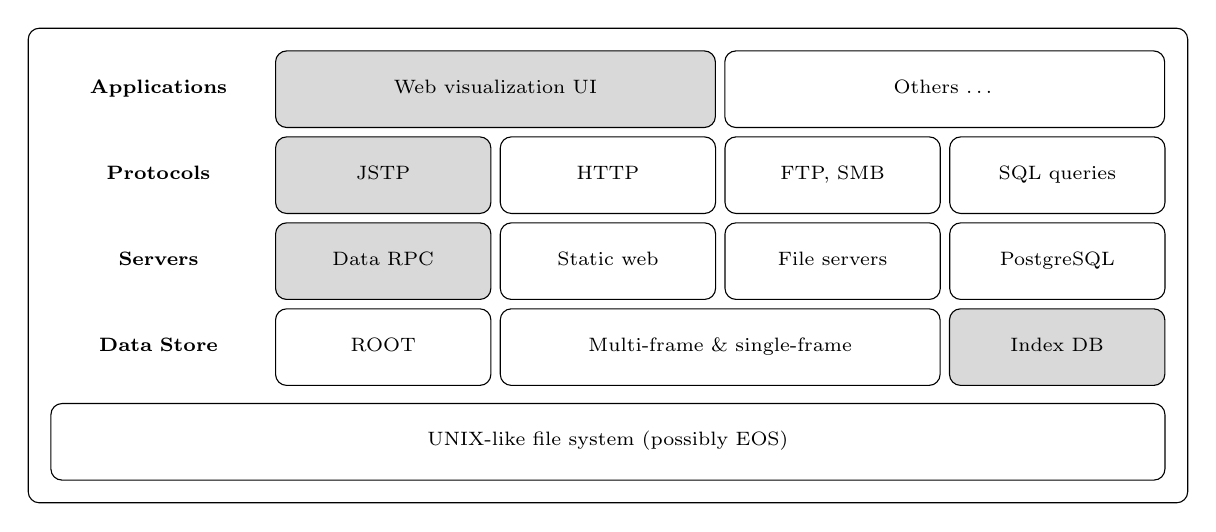
\begin{tikzpicture}[node distance=3pt,
	blueb/.style={
	  draw=black,
	  rounded corners,
	  text width=2.5cm,
	  font=\scriptsize,
	  align=center,
	  text height=12pt,
	  text depth=9pt
	},
	layerb/.style={
	  blueb,
	  draw=none
	},
	proprietaryb/.style={
	  blueb,
	  fill=gray!30
	}]

	\node[layerb] (Clients) {\textbf{Applications}};
	\node[proprietaryb,right=of Clients,text width=5cm+10pt] (VizUI) {Web visualization UI};
	\node[blueb,right=of VizUI,text width=5cm+10pt] (Apps) {Others \dots};

	\node[layerb,below=of Clients] (Protocols) {\textbf{Protocols}};
	\node[proprietaryb,right=of Protocols] (JSTP) {JSTP};
	\node[blueb,right=of JSTP] (HTTP) {HTTP};
	\node[blueb,right=of HTTP] (FileP) {FTP, SMB};
	\node[blueb,right=of FileP] (SQLP) {SQL queries};

	\node[layerb,below=of Protocols] (Servers) {\textbf{Servers}};
	\node[proprietaryb,right=of Servers] (DataS) {Data RPC};
	\node[blueb,right=of DataS] (WebS) {Static web};
	\node[blueb,right=of WebS] (FileS) {File servers};
	\node[blueb,right=of FileS] (SQLS) {PostgreSQL};

	\node[layerb,below=of Servers] (Data) {\textbf{Data Store}};
	\node[blueb,right=of Data] (ROOT) {ROOT};
	\node[blueb,right=of ROOT,text width=5cm+10pt] (MF) {Multi-frame \& single-frame};
	\node[proprietaryb,right=of MF] (SQLD) {Index DB};

	\node[blueb,below=2.4cm of HTTP,text width=13cm+26pt] (FileSystem) {UNIX-like file system (possibly EOS)};

	\begin{pgfonlayer}{background}
	\draw[blueb,draw=black] 
	  ([xshift=-8pt,yshift=8pt]current bounding box.north west) rectangle 
	  ([xshift=8pt,yshift=-8pt]current bounding box.south east);
	\end{pgfonlayer}
	\end{tikzpicture}

\caption[Multi-layered system.]{A multi-layered system. Proprietary components are emphasized by gray color.}
\label{fig:multilayered-diagram}
\end{center}
\end{figure}

This may be illustrated on a practical application. Users who want a quick peek at the detector operation without any effort might decide to use the visualization UI in their web browser. The website is quite easy to use, does not require any particular skills to operate, and is capable of displaying frames captured by the detectors as well as overview of their operation. In contrast, users who want to retrieve data for experimentation or statistical aggregation might utilize SQL or JSTP as these two protocols are not designed to interact with humans, but with other applications, most notably usable in scripts designed for custom data processing. Lastly, users in need of information, which is not displayed by the visualization UI nor transmitted by any of the mentioned protocols, can connect to the database storage facility remotely and directly download data files by means of some of the supported network transfer protocols. This concept is illustrated in Figure \ref{fig:multilayered-diagram}.

% CITACE: konkurenční projekty
JSTP is built with extensibility in mind. With multiple concurrent projects such as MoEDAL-TPX\footnote{Similarly to ATLAS-TPX, MoEDAL-TPX is a network of Timepix devices installed within the MoEDAL experiment at CERN.}, SATRAM\footnote{SATRAM is a technology demonstration device carrying Timepix position-sensitive semiconductor pixel detector on board ESA’s Proba V satellite. \url{http://satram.utef.cvut.cz/}} and RISESat\footnote{RISESat is a microsatellite mission carrying several scientific instruments including a Timepix detector.}, it is likely that JSTP will be used for compatibility reasons in other applications as well. It should therefore allow for limited variability, gracefully handling minor alterations in transmitted data structures.

\subsection{Requirements}
This section lists all formal requirements on JSTP. The most basic requirement is that the protocol allows to retrieve frames captured by the ATLAS-TPX network by their start time and device of origin. This might remind observant readers of a similar requirement stated in the database definition (see section \ref{db:definition}), as it is the most likely user request. However unlike the database, JSTP must be able to transmit only those frames, which satisfy the user predicate, effectively reducing information overhead in transmitted messages to zero.

In the first version, JSTP is required only to transmit results of cluster analysis, leaving door open for pixel matrix transmissions in the future. This indirectly implies that every message transmitted through JSTP containing a captured frame consists of two parts: a header (containing detector configuration, position, orientation, etc.) and a body (containing a list of clusters, or possibly a pixel matrix).

To efficiently reference detectors in the ATLAS-TPX network, it is required that JSTP provides an exhaustive list of network elements along with information about their availability in the system. This might seem redundant at first, but consider that JSTP needs handle situations when detectors malfunction, are replaced, or new detectors are installed. Such events might not be that uncommon, especially given the experimental nature of the project.

Lastly, in order to aid with navigation in large amounts of detector footage, JSTP has to offer a mechanism to generate statistics over larger periods of time. This information will help users find events of interest in overwhelming quantities of white noise, resembling the proverbial \textit{needle in a haystack}.

Apart from various file management network protocols listed earlier, there are no data manipulation requirements on JSTP, implying that the protocol cannot be used for other than read-only access to detector footage.

\section{Underlying Standards}
JSTP is a web protocol and as such, it utilizes HTTP as its underlying standard, serving to abstract physical data transmission and compression. By this declaration, it is implied that JSTP is a request-response communication protocol between two types of agents: \textit{a server} and \textit{a client}.

In its architecture, JSTP consists of two parts: a web service providing API for remote procedure calls (RPC) and a data format built atop of it to facilitate such calls. Since JSTP does not include any universal service description mechanism such as WSDL or WADL, all clients need to know its capabilities and calling conventions prior to initiating communication with the server. For data serialization, JSTP utilizes JavaScript Object Notation (JSON) (hence its name). This format has been selected for various reasons. It is simple to parse, offers an extensible tree structure and is very common among web services of this kind, as it is directly supported by the JavaScript client-side runtime used in the web visualization UI. Apart from JSON, JSTP does not offer nor accept communication in any other data formats.

One might ask whether JSTP web methods meet the standards of RESTful web services. While it is true that the protocol shows many traits often attributed to RESTful services (client-server model, stateless protocol, cacheability, layered system), it certainly does not satisfy all of them. For example, JSTP does not uniquely identify resources by their URI because it does not offer any of the common CRUD operations. Moreover, in referencing entities, JSTP uses arbitrary identifiers (recall members \texttt{fid}, \texttt{frid} and \texttt{sid} of entities defined in section \ref{db:definition}), which are not passed in the URI but through an array in the request body. Moreover, JSTP does not offer a uniform interface, capable of negotiating data format according to client limitations. Instead, it forces clients to communicate strictly in JSON, adhering to its own arbitrary data structures and calling conventions.

\todo % revisions finished to this point

\section{Web Methods}
\label{jstp:web-methods}
The main component of JSTP is a web service, which can be described as a set of proprietary web methods. For the purpose of simplicity, in this section we provide only a semantical description of each method. Readers interested in full technical documentation of the methods are referred to Appendix \ref{apx:jstp-doc}.

\subsection{Detector List}
The first method is dedicated to providing an updated list of operational detectors in the ATLAS-TPX network.

As we mentioned earlier, we need to be ready for situations when the physical structure of the network changes due to malfunctions or upgrades. For these reasons, any client intending to retrieve frames from a specific detector must first consult the list provided by this method to verify, whether the device is still connected and operational. In addition, other clients unaware of the network's architecture may use this method to obtain an exhaustive listing of all currently available data sources.

Execution of this method requires no parameters. The server responds by transmitting a list of devices, from which data can be retrieved at the time of request. For detailed documentation of this method including examples of requests and responses, see section \ref{apx:jstp-sensors} of the Appendix.

\subsection{Overview of Acquisition}
To satisfy demands on navigation in voluminous amounts of data, we dedicate the second web method to providing an overview on detector acquisition. This is achieved by uniformly dividing a specific time period into finitely many time intervals, in which all relevant frames are gathered with respect to their start time (acquisition time is not considered). In every interval, frames are subsequently processed to produce aggregate statistics, which might indicate time points, where frames of interest are located. This approach is in its essence very similar to the binning procedure used when constructing histograms.

Clients calling this method are required to transmit five parameters in their request:

\begin{description}
	\item[Detector Predicate]
	A group of detector identifiers, restricting all processed frames by their device of origin.

	\item[Start Time, End Time]
	These parameters define the time period, in which we generate statistics. Obviously, the first parameter must be an earlier point of time than the latter.

	\item[Group Period]
	The duration of every interval in the partitioning of the time period. Should an imperfect partitioning occur, the number of intervals is always rounded up to the nearest integer, possibly exceeding the specified end time.

	Longer durations obviously result in a lower number of intervals, and in turn a lower number of returned data points. Shorter durations yield more data points, but may result in lengthy processing at server-side. For stability reasons, the server therefore requires that the duration of the group period results in at least 1 and at most 1024 intervals.

	\item[Normalized Mode]
	An option to compensate possible data distortions caused by variations in frame acquisition times. This setting is irrelevant in configurations, where users can be certain such variations do not occur.
\end{description}

If the server finds request parameters to be valid and succeeds in generating requested statistics, it responds by transmitting a list of data points, corresponding with intervals of the partitioning of the specified time period. Every data point includes three values:

\begin{description}
	\item[Cluster Counts]
	Sums of cluster counts from every frame in the interval, summed separately per every of the six cluster types (for type definitions, see section \ref{db:shape-classification}).

	\item[Frame Occupancy]
	Total number of non-zero pixels in all frames in the interval, indicating their levels of saturation.

	\item[Number of Frames]
	The count of frames aggregated in the interval.
\end{description}

For detailed documentation of this method including examples of requests and responses, see section \ref{apx:jstp-timeline} of the Appendix.

\subsection{Frame Search}
The third method serves to retrieve frames captured at any given point in time by a detector (or a group of detectors). As the method's name might suggest, time need not be exact, resulting in a search for the nearest frame operating on the scope of the index database. There are several search modes available, each offering a different strategy to find \textit{the master frame}. Once such frame is identified, its start time is then used to locate other frames from the remaining detectors, yielding at most one frame per every detector. In the first version of JSTP, we support two search modes:

\begin{description}
	\item[Sequential Forward Mode]
	The master frame is the frame with the start time nearest to, but greater or equal than the time parameter of the search.

	\item[Sequential Backward Mode]
	The master frame is the frame with the start time nearest to, but lower or equal than the time parameter of the search.

	%\item[Sequential Omnidirectional Mode]
	%\item[Exact Match Mode]
\end{description}

Let us demonstrate operation of these modes on a real world example. Suppose that we are interested in frames captured by two devices. Detector 1 captures frames every 0.25 seconds with acquisition time of 0.05 seconds, whereas detector 2 captures frames every 0.33 seconds with acquisition time of 0.27 seconds. If we set the search time to 0.4 seconds and search in the forward mode, the third frame captured by detector 1 will be designated as the master frame. Since the start time of this frame is 0.5 seconds, the second chosen frame will be the second frame captured by detector 2 as its start time is 0.33 seconds and its end time is 0.6 seconds. This scenario is depicted in Figure \ref{fig:frame-search-forward}. If we to use the backward mode instead, the second frame captured by detector 2 will be designated as the master frame. Since its start time is 0.33 seconds and there is a gap in detector 1 footage between 0.3 seconds (end time of the second frame) and 0.5 seconds (start time of the third frame), the algorithm will return no frame for the other detector. This is illustrated in Figure \ref{fig:frame-search-backward}.

% TODO: doplnit dva obrázky

\begin{figure}[t]
\begin{center}
	\begin{subfigure}[b]{0.4\textwidth}
	\Large
	\begin{tikztimingtable}
		\textnormal{D1}   & zz D{1}zzzz D{2}zzzz D{3}zzzz ;[fill=yellow!50]D{4};[fill=none] zzzz D{}         \\
		\textnormal{D2}   & zz 5D{1}z ;[fill=gray!30]5D{2};[fill=none]z 2D{}  \\
		\textnormal{D3}   & zz 2D{1}z   2D{2}z   2D{3}z   ;[fill=gray!30]2D{4};[fill=none] z    2D{5}z 0.5D{}   \\
		\extracode
	\begin{pgfonlayer}{background}
	\vertlines[help  lines]{1,9,10,13}
	\end{pgfonlayer}
	\end{tikztimingtable}
	\caption{Forward search.}
	\label{fig:frame-search-forward}
	\end{subfigure}
	~ %spacing
	\begin{subfigure}[b]{0.4\textwidth}\Large
	\begin{tikztimingtable}
		\textnormal{D1}   & zz D{1}zzzz D{2}zzzz D{3}zzzz D{4}zzzz D{}         \\
		\textnormal{D2}   & zz 5D{1}z ;[fill=gray!30]5D{2};[fill=none]z 2D{}  \\
		\textnormal{D3}   & zz 2D{1}z   2D{2}z   2D{3}z   ;[fill=yellow!50]2D{4};[fill=none] z    2D{5}z 0.5D{}   \\
		\extracode
	\begin{pgfonlayer}{background}
	\vertlines[help  lines]{1,8.5,9,13}
	\end{pgfonlayer}
	\end{tikztimingtable}
	\caption{Backward search.}
	\label{fig:frame-search-backward}
	\end{subfigure}

\caption{Time diagram of frame search illustrating behavioral differences between search modes. Individual blocks correspond with periods of detector acquisition. Emphasized blocks are returned as the search result (yellow marks the master frame).}
\label{fig:frame-search}
\end{center}
\end{figure}

To summarize, clients calling this method are required to specify four parameters:
\begin{description}
	\item[Time of Search]
	The point in time used as a starting point of the search.

	\item[Detector Predicate]
	A group of detector identifiers, restricting retrieved frames by their device of origin.

	\item[Search Mode]
	A strategy to select the master frame based on the time of search and available detector footage.

	\item[Integral Frames]
	Number of consecutive frames to be integrated for every device.
\end{description}

If the server finds request parameters to be valid and succeeds in locating at least one frame, it responds by transmitting the start time of the master frame, followed by headers and bodies of all found frames, corresponding with the order of identifiers in the detector predicate of the request. Frame bodies are transmitted in the form of cluster lists (for properties of clusters, see section \ref{db:cluster-properties}). Detailed documentation of this method, including examples of requests and responses, is available in section \ref{apx:jstp-frame} of the Appendix.

\section{Miscellaneous}
JSTP has been originally designed to serve solely as a data transmission component of the visualization UI. Over time, it has however grown to be a more complex protocol, with applications in other projects than ATLAS-TPX and outside the conventional task of data visualization. It is the intention of author to continue development of this protocol with further releases in the future, eventually decoupling it from the Timepix chip and abstracting it to the point where it could be utilized in combinations with different hardware.

Since the amount of data in our database is expected to become rather overwhelming, the protocol itself is structured and meant to be used in a top-down model (see Figure \ref{fig:jstp-uml}), allowing clients to gradually refine parameters of their requests and locate the information they seek, while avoiding transmission of data in overly granular bulks. In other cases, the protocol minimizes information overhead by requiring strong usage of predicates operating on the index database.

Note that in the protocol definition, we do not specify whether the results of individual web method calls are cacheable by clients. This is due to the diversified nature of its applications. Since HTTP already contains its own caching logic\footnote{Caching in HTTP is controlled by values of headers provided in every response message. Relevant header names are: \texttt{Cache-Control}, \texttt{Expires} and \texttt{Pragma}.}, we encourage all clients to comply with strategies described in \cite{HTTP1999}, section 13, as JSTP servers are permitted to use this mechanism to emply different caching policies for individual response messages. Analogous declaration is used for data compression (for HTTP specification, see section 3.5 of \cite{HTTP1999}).

\begin{figure}[t]
\begin{center}
	\begin{sequencediagram}
		\newthread{c}{:JstpClient}
		\newinst[2]{s}{:JstpServer}
		\newinst[1]{idb}{:IndexDatabase}
		\newinst{fdb}{:FileDatabase}

		\begin{call}{c}{detectorList()}{s}{device list}
			\begin{call}{s}{selectSensors()}{idb}{device list}
			\end{call}
		\end{call}
		
		\begin{sdblock}{Until significant data is found}{}
			\begin{call}{c}{acqOverview()}{s}{statistics}
				\begin{call}{s}{selectFiles()}{idb}{affected files}
				\end{call}
				\begin{call}{s}{selectFrames()}{idb}{statistics}
					\begin{callself}{idb}{\small aggregate()}{}
					\end{callself}
				\end{call}
			\end{call}
		\end{sdblock}
		
		\begin{call}{c}{frameSearch()}{s}{found frames}
			\begin{call}{s}{selectFrames()}{idb}{master frame}
			\end{call}
			\begin{sdblock}{For every device}{}
				\begin{call}{s}{selectFrames()}{idb}{entry indices}
				\end{call}
				\begin{call}{s}{readFile()}{fdb}{frame contents}
				\end{call}
			\end{sdblock}
		\end{call}
	\end{sequencediagram}

\caption{UML diagram depicting expected interactions between JSTP client and server, hinting levels of processing complexity at server-side.}
\label{fig:jstp-uml}
\end{center}
\end{figure}










\chapter{Server Implementation}
\label{chapter:server}
This chapter describes the implementation of a web application, most notably responsible for the web visualization UI.

\section{Decomposition}
The server application consists of two major components, a JSTP data server and a static web server. As their names suggest, the data server asynchronously delivers data to be visualized in the form of JSTP messages, whereas the web server provides the visualization UI in the form of static-hosted files.

Both applications run simultaneously and independently of each other as Linux daemons or services in an initialization system, communicating only by means of network sockets. Each application listens and responds to client requests on its own dedicated port.

\subsection{JSTP Data Server}
The JSTP data server is a C++ application built using the Facebook Proxygen open source library\footnote{For more information, see project website: \url{https://github.com/facebook/proxygen}}. It is responsible for interacting with the ATLAS-TPX footage database and the index database, in order to transcode TPX footage into the JSTP format.

The core component of the server is a thread pool. It allows simultaneous communication with multiple clients, provided that the server's hardware offers parallel processing support. At the startup, multiple \textit{worker threads} are created. These threads are immediately suspended to conserve server's resources. When a new request arrives, one of the suspended threads is awakened and notified to process the request and compose a response, which is then transmitted back to the client. During this operation, the thread is said to be \textit{busy} and cannot receive new requests until the processing is completed. Should a new request arrive at that time, the server would opt to awaken another of the suspended threads, gradually exhausting its pool. After a response is sent, the busy thread returns to a suspended state, awaiting further instructions. This way, threads are recycled within the pool throughout server operation.

\subsection{Static Web Server}
The web server is a standard server application implemented in Node.js. It stores all files and dependencies of the web visualization, such as HTML files with UI definition, style sheets written in CSS and client-side scripts written in JavaScript. Since these files are quite static in their essence, the web server uses standard HTTP caching mechanisms to speed up its operation.

For security reasons, the HTTP socket managed by the web server is the only socket accessible from the Internet. All JSTP traffic is routed through this socket and then redirected to a private socket owned by the JSTP server, eliminating the need to expose more than one port to the Internet.

\section{Object-Oriented Design}
In the JSTP data server, much emphasis was put on the object design and the use of standard design patterns. \cite{DesignPatterns} This section contains the most notable instances.

\subsection{Request Handling}
When a request arrives, a worker thread is assigned to process it and respond accordingly. To avoid keeping all server logic inside implementation of worker threads, the process of producing a response to a single instance of a request is genereated by \textit{a request handler}.

When the worker thread determines, which JSTP method is called, a corresponding request handler is created, and given abstracted control over the HTTP socket. After the handler has finished processing the request, the worker thread sends the response to the client and destroys the handler, freeing resources related to the communication session.

Using object polymorphism, multiple types of request handlers are implemented to service requests corresponding with various JSTP web methods listed in section \ref{jstp:web-methods}.

\subsection{Behavior Selection}
Apart from producing server responses, the worker threads are also responsible for choosing the appropriate behavior for every client request. In comparison to processing requests themselves, this logic consists mostly of picking the correct request handlers. Thus, it is autonomous by the application of the factory method design pattern (see Figure \ref{fig:handler-factory}). \cite{DesignPatterns}

When started, every worker thread creates \textit{a factory} object. This object is later called when requests arrive, and, based on their parameters, determines which request handler shall be used in order to produce a response.

Since the JSTP specification uses URL to determine the called web methods (and by extension request handlers), a factory subclass utilizing regular expressions to perform decisions about requests was implemented. At the creation time of the subclass, all supported request handlers along with their respective regular expressions are registered using the standard builder design pattern. One more request handler is designated as \textit{the default handler}. Upon request, all of the registered expressions are matched on its URL sequentially. Should one of them succeed, its corresponding request handler is selected. Otherwise, the default handler is used to inform the user of an invalid request.

\begin{figure}[t]
\begin{center}
	\begin{tikzpicture}
		\begin{abstractclass}[text width=7cm]{HandlerFactory}{0,0}
			\operation[0]{+ createHandler ( req : HTTPRequest )}
		\end{abstractclass}

		\begin{abstractclass}[text width=7cm]{RegexHandlerFactory}{0,-3}
			\inherit{HandlerFactory}
			\attribute{- handlers : RequestHandler[0..*]}
			\attribute{- expressions : RegularExpression[0..*]}
			\attribute{- defaultHandler : RequestHandler}
			\operation{+ createHandler ( req : HTTPRequest )}
			\operation[0]{\# registerHandlers ( )}
		\end{abstractclass}

		\begin{class}[text width=5cm]{JSTPHandlerFactory}{8,-5}
			\inherit{RegexHandlerFactory}
			\operation{\# registerHandlers ( )}
		\end{class}

		\begin{class}[text width=3cm]{HandlerA}{6,0}
			\operation{+ process ( )}
		\end{class}

		\begin{class}[text width=3cm]{HandlerB}{10,0}
			\operation{+ process ( )}
		\end{class}

		 \draw[umlcd style dashed line,->] (JSTPHandlerFactory) --node[above,sloped, black]{$<<$instantiate$>>$} (HandlerA);
		 \draw[umlcd style dashed line,->] (JSTPHandlerFactory) --node[above,sloped, black]{$<<$instantiate$>>$} (HandlerB);
	\end{tikzpicture}

\caption[UML diagram illustrating handler instantiation.]{UML diagram illustrating the abstract factory design pattern applied in the context of request handler instantiation.}
\label{fig:handler-factory}
\end{center}
\end{figure}

\subsection{Content Abstraction}
In order to produce valid JSTP messages, a JSON serialization component is required. All web methods are expected to read their parameters and compose their responses in the desired format. Since this behavior is shared amongst all request handlers, it is encapsulated in a separate subclass of a conventional request handler. To access properties of this subclass, all request handlers corresponding to JSTP web methods inherit from it.

The subclass interacts directly with the HTTP socket and uses \textit{a parser} and \textit{a writer} to retrieve and produce JSON strings. Its descendants can thus only call the parser and the writer to access and produce content, instead of reading and writing to the socket directly, as illustrated in Figure \ref{fig:request-handlers}. This prevents bad object design by centralizing serialization logic in a single object. In addition, it allows for a limited degree of variability, since the subclass itself is the sole object responsible for communicating information to the socket.

\begin{figure}[t]
\begin{center}
	\begin{tikzpicture}
		\begin{abstractclass}[text width=5cm]{RequestHandler}{0,0}
			\attribute{\# socket : HTTPSocket}
			\operation[0]{+ process ( )}
		\end{abstractclass}

		\begin{abstractclass}[text width=5cm]{JSONRequestHandler}{0,-3}
			\inherit{RequestHandler}
			\attribute{\# writer : JSONWriter}
			\attribute{\# parser : JSONParser}
			\operation[0]{+ process ( )}
		\end{abstractclass}

		\begin{class}[text width=3cm]{HandlerA}{6,-2}
			\inherit{JSONRequestHandler}
			\operation{+ process ( )}
		\end{class}

		\begin{class}[text width=3cm]{HandlerB}{6,-4}
			\inherit{JSONRequestHandler}
			\operation{+ process ( )}
		\end{class}
	\end{tikzpicture}

\caption[UML diagram illustrating handler inheritance.]{UML diagram illustrating the inheritance of request handler objects.}
\label{fig:request-handlers}
\end{center}
\end{figure}

\section{Performance Optimizations}
In the JSTP server, various performance optimizations are used to minimize response latency. This section lists some of these optimizations.

\subsection{ROOT Reading Optimization}
It was shown in section \ref{storage:ROOT} that the ROOT format stores information in tree structures, separatingthe detector configuration from the cluster lists corresponding to individual frames. Due to possibly overwhelming sizes of data files, it is nontrivial to devise a logic to minimize access time with respect to memory paging and L1 cache. Some of the most significant factors to consider are:

\begin{description}
	\item[ROOT Compression]
	The ROOT data format utilizes its own compression algorithm, roughly equivalent to the ZIP format in its efficiency. There are multiple levels of compression ranging from the best compression ratio to the fastest reading time. The choice of the compression level affects all subsequent processing required to encode and decode data.

	\item[ROOT Cache]
	The ROOT data format implicitly uses a file cache to prefetch information in memory with the assumption that the data will be read sequentially. For that reason, linear enumeration of data structures tends to be faster than a random access.

	\item[Tree Locality]
	When retrieving frame data, switching from the \texttt{dscData} tree to the \texttt{clusterFile} tree and back might cause OS to swap memory every time a single frame is read, producing unnecessary overhead and slowing down the process.

	\item[Data Demand]
	In many instances of JSTP messages, it is requested that only a portion of the stored data is read. ROOT allows applications to specify this information prior to initiating sequential reading, and in turn accelerate some procedures.
\end{description}

With respect to the these factors, all instances of objects requiring to read data from the ROOT file format, do so sequentially in strides. The application producing ROOT data files is configured to use the medium compression level, offering acceptable access speeds while maintaining a good compression ratio.

When reading frame data, all configuration information is first read from the \texttt{dscData} tree. After the information is processed, the server moves on to the \texttt{clusterFile} tree and repeats the procedure without returning to the \texttt{dscData} tree in the process to prevent unnecessary swaps and utilize benefits of ROOT cache. Lastly, all components of the server interacting with the ROOT file format exhaustively declare, which tree branches are subject to processing later on.

\subsection{Centralized File Management}
In the web visualization UI, users may often browse frames in the order of acquisition. If a naive implementation was used, this would imply that on the server-side the same ROOT file is opened, read from and closed multiple times over. Such behavior would be unnecesarily wasteful, as the procedure of opening and closing file pointers to possibly large files may become somewhat inefficient, and in turn slows down the server operation significantly.

To resolve this problem, a centralized data structure is introduced into the JSTP server. This structure is accessible to other components (such as request handlers) in compliance with the singleton design pattern. Its main responsibility lies in opening and closing ROOT files, with which the other components interact. Its implementation however does not forward these calls directly to the file system. Instead, an internal time-driven caching mechanism is used to recycle open file pointers between multiple consumers according to their needs. The pointers are closed only when their contents are no longer requested for a greater period of time.

A central structure shared amongst multiple components operating on different threads does not induce a race condition, because it allows multiple instances of the same file to be open at the same time. Two threads requesting the same file in parallel would thus not need to wait on each other.

\section{User Interface Documentation}
The web visualization UI consists of a single static HTML page, which is provided to the users by the web server. Apart from UI definitions and style sheets, it includes several client-side scripts, controlling the behavior of the website in the web browser. From a design standpoint, the UI is divided into multiple sections (depicted in Figure \ref{fig:wireframe}), each with a dedicated role and purpose.

\begin{figure}[t]
\begin{center}
	\begin{tikzpicture}[
	section/.style={
	  rectangle,
	  draw=black,
	  font=\scriptsize,
	  align=center,
	  inner sep=0pt,
	  fit=#1
	}]
		\coordinate (A) at (0,0);
		\coordinate (B) at (15,-1);
		\coordinate (C) at (0,-1);
		\coordinate (D) at (15,-3);
		\coordinate (E) at (10,-3);
		\coordinate (F) at (15,-10);
		\coordinate (G) at (0,-3);
		\coordinate (H) at (10,-9);
		\coordinate (I) at (0,-9);
		\coordinate (J) at (10,-10);

		\node (header) [section={(A) (B)}] {Header};
		\node (timeline) [section={(C) (D)}] {Overview Chart};
		\node (details) [section={(E) (F)}] {Details};
		\node (frame) [section={(G) (H)}] {Main Chart};
		\node (status) [section={(I) (J)}] {Status};
	\end{tikzpicture}

	\todo % Screenshot?

\caption{Wireframe showing the layout of UI sections.}
\label{fig:wireframe}
\end{center}
\end{figure}

\subsection{Header Bar}
The uppermost section of the UI is dedicated to important descriptive and control elements of the screen. From the left to the right, it contains the logos of the institutions involved in the data acquisition, detector control box, time control box and a frame stepper.

\begin{description}
	\item[Institution Logos]
	This section includes the logos of the ATLAS collaboration, Institute of Experimental and Applied Physics and the Czech Technical University in Prague. All pictures are linked to the respective institution websites.

	\item[Detector Control]
	The detector control box allows users to specify a device (or a set of devices) in the ATLAS-TPX network to be used as a data source for the displayed frames. If only one device is selected (the default configuration), the box is optimized to allow quick switching using a dropdown control and incremental toggle buttons on its sides.

	\item[Time Control]
	This box controls the start time of the displayed frames. It is essentially a simple date input element with additional incremental toggle buttons for every component of the date.

	\item[Frame Stepper]
	This control is a simple extension of the time control box, allowing users to quickly browse frames sequentially in order of their acquisition. It consists of two big buttons with arrows pointing left and right, signifying the direction of time movement. Next to these buttons, a number input element is located. This element is responsible for controlling the number of integral frames.
\end{description}

\subsection{Overview Chart Area}
The overview chart is placed below the header bar and fills the entire width of the screen. Its purpose is to inform the users about detector acquisition in a determinate time period, referred to as \textit{the window}. To facilitate the navigation in the data, the chart shows a vertical line at the point corresponding to the current start time of the displayed frames. Upon every change of this parameter, the line moves horizontally in the chart to adjust. Should the line be plotted out of bounds by leaving the chart either on the left or the right side, the window is automatically updated to compensate. It is worth noting that this mechanism also works the other way around. Users can set the start time of the displayed frames to any time point from the window by clicking at its respective position on the horizontal axis.

In the chart, multiple series are plotted simultaneously. The horizontal axis always corresponds to time, whereas the vertical axis may correspond to the number of clusters, flux or frame occupancy, depending on the series in question. There are at most 8 plotted series at any instance. Their appearance is described by the legend located in the bottom left part of the chart area. Apart from providing description on the displayed series, the legend also allows users to turn plotted series on or off by clicking on the respective items of the legend. The series can be semantically divided in three groups:

\begin{description}
	\item[Cluster Counts]
	The cluster rate is shown separately for the different cluster types (shown in section \ref{db:shape-classification}). These series have no unit as their values merely correspond with the number of clusters occupying frames, whose start time falls into a specific time interval.

	If the normalized mode is active, contributions to these series from every frame is first divided by the acquisition time of the frame, producing flux values with unit $s^{-1}$.

	\item[Total Sum]
	This series plots the sum of cluster counts over all cluster types. Its unit is same to that of the previous six series.

	\item[Frame Occupancy]
	The values of this series correspond to the portion of frame area occupied by non-zero pixels. It has no unit and is distinguished from the other series by a dashed line. 
\end{description}

The overview chart offers a number of custom settings. The length of the window can be reconfigured to any value from 30 seconds to 4 days by controls located in the bottom right corner of the chart area. The window itself can also be adjusted to align the vertical line corresponding to the current start time of displayed frames to the center of the screen. Furthermore, the chart offers two rendering modes to choose from:

\begin{figure}[t]
\begin{center}
	% TODO: use vector picture for this
	% tpx01 @ 2016-04-08 23:36:28.012, window = 2h

	\begin{subfigure}{\textwidth}
	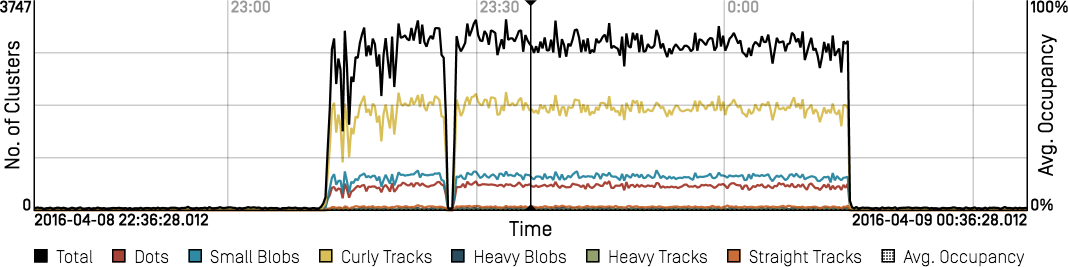
\includegraphics[width=\textwidth]{figures/overview-absolute}
	\caption{Absolute mode.}
	\label{fig:overview-chart-absolute}
	\end{subfigure}

	\vspace{0.2cm}

	\begin{subfigure}{\textwidth}
	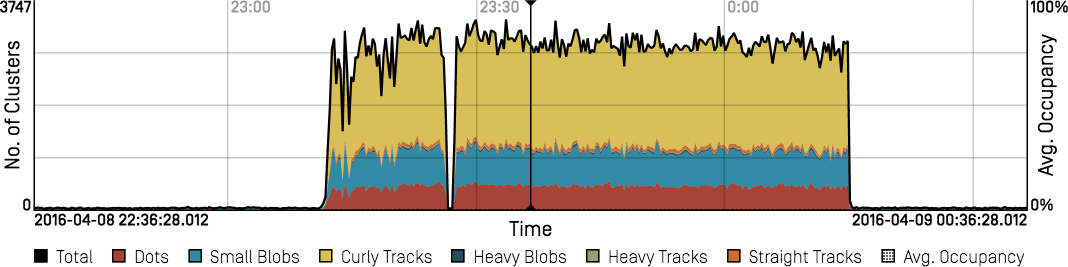
\includegraphics[width=\textwidth]{figures/overview-stacked}
	\caption{Stacked mode.}
	\label{fig:overview-chart-stacked}
	\end{subfigure}

\caption[Comparison of overview rendering modes.]{Example of the same overview chart rendered in different modes.}
\label{fig:overview-chart-modes}
\end{center}
\end{figure}

\begin{description}
	\item[Absolute Mode]
	In this mode (seen in Figure \ref{fig:overview-chart-absolute}), all series of the chart are rendered as points in the plane with respect to the horizontal and vertical axis. Consecutive points of every series are connected by line segments of different color to indicate continuity in time.

	This mode enables users to easily compare values of different series to each other. However, since the experimental data often includes one or two prevailent series, it also frequently overshadows the remaining series as they are rendered over each other, making it harder to read their values.

	\item[Stacked Mode]
	In this mode (seen in Figure \ref{fig:overview-chart-stacked}), the six series corresponding to cluster counts are rendered in a stacked chart, cumulatively adding to each other. Each cluster type series corresponds to a colored area in the chart, while the remaining series are rendered in the same way as in the absolute mode.

	In comparison to the previous mode, this mode distorts the absolute values of the series. It however much better portrays the ratio of representation of one series to another, especially in situations when series have similar values.
\end{description}

\subsection{Main Chart Area}
As the name suggests, the main chart area is the primary section of the UI dedicated to plots of frames from the TPX detectors. By default, it shows only data from a single detector. It can however be configured to partition itself into multiple \textit{cells}, each corresponding to data acquired by a different detector in the network. This feature is often useful on large screens and projectors.

Each cell consists of two square charts, corresponding to individual sensor layers of the detector. Both charts are identical in their layout and internal structure, differing only in the data visualized. Since frames are in their essence pixel matrices, charts visualize them in a standard way by mapping pixel values to different colors, which are later used to fill rectangular areas in the chart. Frame charts can be customized in several ways:

\begin{description}
	\item[Visualized Values]
	If a visualized frame has been captured in the TOT mode, calibration method described in \cite{EnergyCalibration} can be used to obtain energy values from raw counter values. In other operation modes, only counter values are available.

	By default, both charts visualize energy values in the TOT mode and counter values in the other modes. This setting can however be overridden to always visualize counter values in all modes instead.

	\item[Scale Bounds]
	In order to map pixel values to colors, a determinate interval must be specified to establish scale bounds. This interval is by default calculated from the visualized frame automatically. Users can configure its bounds to any fixed values by deactivating the \textit{auto range} checkbox in the details panel.

	\item[Scale Types]
	Given specific scale bounds and values of individual pixels, any function can be used to map absolute values to relative values from a $[0;1]$ interval. By default, a simple linear mapping is used for this task. Users can change this setting to a logarithmic mapping, which better accentuates order differences between individual pixel values in some frames.

	\item[Color Themes]
	The choice of color corresponding to a value between zero and one is purely arbitrary. The visualization UI offers three color themes commonly used in other research programs:

	% CITACE: http://matlab.izmiran.ru/help/techdoc/ref/colormap.html
	\begin{itemize}
		\item The \textit{Jet} theme ranges from blue to red, and passes through the colors cyan, yellow, and orange.
		\item The \textit{Hot} theme varies smoothly from black through shades of red, orange, and yellow, to white.
		\item The \textit{Gray} theme returns a linear grayscale ranging from black to white.
	\end{itemize}
\end{description}

Apart from the listed customizations, frame charts show interactive data labels by responding to mouse movements over the chart area. When the mouse enters the frame, two perpendicular lines are drawn on the pixels underneath the mouse cursor. These lines track the cursor while it hovers over the chart. In addition, several rows of descriptive information are displayed next to the intersection of the lines, giving details on the pixel values and various properties of its associated cluster.

Furthermore, frame charts offer a simple zooming feature. When hovering over the frame area, users can use the drag-and-drop mouse gesture\footnote{The drag-and-drop gesture consists of depressing the left mouse button, dragging the mouse while still holding the button down and then releasing it at a desired position.} to highlight a square portion of the frame. Bounding line segments of this square are then set as the new bounds of the horizontal and vertical axes of the chart. To zoom back, users need to double-click on any position in the frame area.

\subsection{Details Panel}
The details panel is located on the right of the main chart area and consists of multiple auxiliary screens, mostly dedicated to providing further details on the information displayed to the left. The panel is controlled by tabs on the top, each corresponding to a single screen. Only one tab can be selected at any instance. This tab is then highlighted and the respective screen is displayed underneath it.

\begin{description}
	\item[Statistics Screen]
	The statistics screen provides a detailed statistical overview of the currently plotted frames. Should multiple detectors be selected for visualization, it offers an option to select one of the devices as a data source for the overview.

	The statistics consist of two tables. The first table contains cluster counts, calculated on separate rows for every cluster type. Next to the number of clusters, a flux column is displayed. At the bottom of the table, values from both columns are summed together, producing a grand total.

	The second table is displayed only in cases, when the frame has been captured in the TOT mode. It includes a sum of energies from all clusters in the frame and average evergy per cluster with a flux column. At the bottom of the table a calculation of instantaneous luminosity from the number of clusters is displayed. This calculation however makes only sense in frames, which are not fully saturated.

	By default, data from both sensor layers are used in the statistical computations. User may however opt to differentiate statistics by individual sensor layers, doubling the amount of figures in both tables.

	\item[Information Screen]
	The information screen displays configuration of the current detector. Similarly to the statistics screen, when multiple detectors are selected, it offers an option to select one of the devices as a data source.

	The displayed information is grouped in several sections. The first section displays time information, such as the start time and the acquisition time of the frame. The following section displays technical information, for example operation mode, frequency of the TPX clock signal and a unique identification of the chip used to capture the frame.

	The last two sections contain secondary information, such as the position and orientation of the detector within the ATLAS machine, or the index information of the ROOT data file, from which the displayed frame has been extracted.

	\item[Filter Screen]
	The filter screen does not show any information. Instead, it allows users to modify displayed data by setting arbitrary predicates. Since most of such predicates operate on numerical measures (for detailed listing, see section \ref{db:cluster-properties}), they can be specified by defining a minimum and maximum value.

	For convenience, each predicate has an additional switch, which determines if it is active on the current data set. Furthermore, user can activate \textit{the warn mode}, in which a contrasting color is used to highlight all pixels violating the set predicate instead of hiding them.

	When any of the predicates is active, it is not only applied on the displayed charts in the main chart area, but also on the figures displayed on the statistics screen. This is convenient for many applications. To avoid possible confusion, every time predicates are active, a notice is displayed above the statistics screen informing that the values are calculated from only a portion of the frame data.

	In addition to numeric predicates, clusters can be also filtered by shape classification (or by location on pixel matrix). This filtering is achieved by selecting permitted cluster types (or matrix regions) from an exhaustive list of all possible options.

	\item[Settings Screen]
	Similarly to the filter screen, the settings screen does not display any additional information to the user. It merely serves to configure the visualization of the data by enabling or setting various options of the charts.
\end{description}

\subsection{Status Bar}
As in most UI applications, the status bar is located at the very bottom of the screen. Its primary purpose is to inform users of the current state of the visualization, most notably whether a data download is in progress, or whether the visualization is ready for new commands.

To display more information, users can activate \textit{the time profiling mode}, in which every procedure is measured and the time is displayed in the status bar.

\todo
% Revisions finished up to this point.

\section{Plotting Optimizations}
Since rendering of all charts in the application occurs on the client side, where hardware performance is not guaranteed, the web visualization UI attempts to improve the rendering process as much as possible. This section lists few notable examples of methods used to minimize rendering latency and improve the overall appearance of the plotted output.

\subsection{Prerendering}
Both frame charts and the overview chart offer interactive features. For that reason, they often require to be redrawn upon various user-generated events, such as mouse cursor movements or mouse clicks. Since re-rendering of an entire chart could represent a time-consuming operation, especially on computers with weak hardware, optimization of this procedure is required.

Observant users of the visualization could have noticed that often enough, only a portion the charts in question needs to be redrawn. This can, for instance, be demonstrated on one of the frame charts. When the user's mouse is hovering over the chart, two perpendicular lines forming a cross are to appear and track its movements. That would imply that the entire chart is redrawn every time the mouse moves. However, the mouse movement does not affect the data plotted in the chart in any way. To exploit this observation, the chart, which was originally rendered as a whole on a single canvas, is divided into multiple auxiliary canvases, each of them responding to different events.

The auxiliary canvases are transparent, have the same size as the original chart and are laid on top of each other like layers in a photo editor. In addition, every auxiliary canvas maintains an additional bit value signifying whether its state is \textit{valid}. The validity of a canvas can be defined in this context as the state of synchronization between the information drawn on the canvas and the data, which is used to generate such information. Upon different events, some of the auxiliary canvases are invalidated (meaning that their validity bit is set to the \textit{invalid} value). Later on, when the chart is requested to be re-rendered, only those auxiliary canvases, which are invalid, are actually redrawn, saving processor time spent for drawing the remaining canvases.

This technique speeds up the chart rendering significantly, as only portions of charts are redrawn due to UI events. It also implies that every event that affects rendering of UI elements has to come with additional information specifying, which auxiliary canvases need to be invalidated. However, with semantical division of the chart (such as partitioning into data area, scale labels and the mouse cross), this does not seem a complicated task.

\subsection{Pixel Drawing}
One of the UI bugs which proved quite tedious to resolve involved colored rectangles drawn to represent individual pixels of a TPX detector. Given the possibility of zooming, every frame chart has to be able to plot at least $2\times 2$ and at most $256\times 256$ of such pixel rectangles. Since dimensions of the charts adapt to the dimensions of the browser window, every time the window is resized, new dimensions of pixel rectangles need to be calculated.

This calculation is fairly straightforward, but since it utilizes floating-point arithmetic, its results may happen to be imprecise in some cases. And due to this imprecision, pixel rectangles in frame charts used to suffer from periodical fractional offsets, which manifested themselves in the form of a thin grid.

To resolve this issue, the auxiliary canvas responsible for data plots is automatically scaled to size, which is slightly greater than the actual amount of pixels available for rendering, but is a multiple of the number of detector pixels to plot. Consequently, the calculated pixel rectangle dimensions are integer values, and thus allow the usage of \textit{the ImageData API}\footnote{The ImageData API is a part of HTML Canvas API, which allows its users to render pictures by setting values of color components of individual pixels in the bitmap. This approach is faster than the conventional API and guaranteed to not use antialiasing. For more information, see section 4.12.4.2.16 of \cite{HtmlStandard}.}. After the pixels are rendered in the canvas, it is scaled back down to the exact size of the plot area. At this point, antialiasing is performed. However, since the canvas has already been filled with colored rectangles, there are no transparent pixels from which a grid-like structure could be formed. For that reason, a conventional antialiasing algorithm will produce a satisfying picture.

\subsection{Subpixel Rendering}
To render all charts sharply, subpixel rendering is supported. Screens with standard pixel resolutions map logical pixels (referenced by the software) to physical pixels (present in the hardware) bijectively. In comparison, high resolution screens divide their logical pixels uniformly in a way, such that a single logical pixel is displayed by multiple physical pixels. The ratio between these two values is defined in the HTML 5 standard \cite{HtmlStandard} as \texttt{devicePixelRatio}\footnote{For instance, Retina display of Apple iPhone 4 has physical resolution $960\times 640$ and logical resolution $480\times 320$. Its pixel ratio is therefore 2.}.

When determining chart sizes prior to rendering, the visualization UI reads the value of the pixel ratio of the current screen and uses it as a coefficient to upscale all canvases accordingly. Contents of charts are then drawn on the canvases, utilizing the enhanced resolution of the screen.

\section{Deployment}
Because the server application consists of two independent daemons, each operating on a different platform, a dedicated deployment method is used. In this section, such method is described in detail.

\subsection{Extension Script Translation}
For coding comfort, the website source makes use of extension languages such as LESS or TypeScript. These languages are respective extensions of the standard CSS and JavaScript, implementing useful features, which are missing or are not supported by their base counterparts. However, since ordinary web browsers are not capable of parsing their advanced syntax, all LESS and TypeScript source files need to be translated by a third-party tool before the web application can be deployed.

The products of the translation process are further optimized for deployment by the process of minification, which removes source code comments, white spaces and obfuscates variable and method names in order to compress file size. Since the code is separated into multiple files, such files are concatenated to minimize the amount of HTTP requests needed to fully load the visualization UI. At the end of this procedure, two compressed files in CSS and JavaScript are generated.

\subsection{Bower Dependencies}
The web application utilizes various open source libraries, most notably jQuery and the Bootstrap Framework. To manage all such dependencies in a well arranged way, the Bower dependency management system is used. The web visualization specifies a \textit{Bower manifest file} in the JSON format. This file lists all dependencies as well as their minimum compatible versions.

When the visualization is deployed, the Bower tool is executed to fetch the latest versions of the required libraries and add their redistributable resources to website contents. This process is deeply integrated with the extension script translation, as the redistributable resources are concatenated with other stylesheets and scripts and minified together. Some dependencies even support strongly-typed bindings in TypeScript. These bindings are downloaded along with the redistributable resources and are used to validate client-side scripts during the translation phase.

\subsection{Grunt Build System}
The Grunt system links all deployment phases together. In a way similar to Makefile, it allows target-driven execution of tasks with possible dependencies and variable arguments. This system is also integrated with the standard Node.js package manager application. To deploy the web visualization UI on the server, two main targets are defined in the application's \textit{Gruntfile}:

\begin{description}
	\item[Production Target]
	The primary purpose of this target is to deploy the web visualization UI with maximum emphasis on speed optimization. All possible files including dependencies are concatenated and minified to minimize loading time of the website in the production environment.

	\item[Debug Target]
	This target is not intended for production use. Its purpose is to maximize readability of the code for the purposes of debugging and development. To achieve this effect, several build phases such as minification and obfuscation are skipped.
\end{description}

\section{Data Import}
Since the JSTP server uses the index database to locate data files based on any given start time, all data files subject to visualization must be stored in the ROOT format and referenced in the \texttt{rootfiles} SQL table.

Accounting for the ever-growing nature of ATLAS-TPX footage, a periodical prodcedure needs to be performed every time new data arrives from CERN, in order to keep the visualization UI up-to-date. At the time of writing this work, this procedure is semi-automated and initiated manually every day by the researchers at IEAP.

\subsection{Processing Stages}
At CERN, the control PC generates raw data files from the read-out interface of every detector in the network. Data is produced on a hourly basis and saved in the form of multi-frame files. Using FTP, these files are transferred into a temporary directory on the target hard drive. When all file transfers are completed and the validity of files is confirmed, several scripts designed to check consistency of detector acquisition are executed. These scripts analyze contents of received files, reading common configuration values such as the acquisition time or bias voltage, and attempt to find variations between individual frames.

Should these scripts succeed in detecting suspicious values, the files in question are moved into a separate directory and await further inspection by researchers. Otherwise, they move on to the next stage of processing. In this stage, captured frames are subjected to the cluster analysis (for more information about this process, see section \ref{intro:cluster-analysis}). Should the frames be captured in the TOT mode, at this point calibration data is used in combination with the method described in \cite{EnergyCalibration} to calculate energy values. At the end of this process, ROOT files are produced.

Since the original multi-frame files are not needed anymore, they can be discarded without data loss (or compressed for the purposes of long-term archiving). The ROOT files are moved from the temporary directory to their final location on the hard drive containing the ATLAS-TPX footage database. Subsequently, a dedicated instance of the JSTP data server application is configured to generate information in the index database, in effect registering them for retrieval of JSTP information. From this point onward, the JSTP server as well as the web visualization UI are able to read frames stored within newly added files.

\subsection{Automation of the Procedure}
\label{import-automation}
At the present time, the procedure of extending TPX database with new footage is time-consuming as its processing stages often perform similar operations repeatedly for different purposes. For example, a single enumeration of multi-frame files should suffice both for consistency checking and cluster analysis. Furthermore, index data corresponding with produced ROOT files can be generated at the time of their production.

It is however worth noting that this procedure was originally designed in the fall of 2015 with the sole purpose of transferring data from CERN to IEAP. Its automation is currently under investigation.

\chapter{Web Visualization}

% 5. Webová vizualizace
%  - Původní schéma dekompozice úlohy, problémy s propustností meziprocesové komunikace a parsing overhead.
%  - Finální schéma dekompozice, přesměrování paketů na úrovni socketu.
%  - Zrychlení statické části pomocí cache, protokoly a robustnost aplikace.
%  - Zapojení jazyků LESS a TypeScript pro usnadnění vývoje webu.
%  - Použití systému pro modulární sestavení Grunt a systému pro závislosti Bower.
%  - Tvorba vykreslovacích komponent pro grafové části pomocí HTML 5.
%  - Integrace komponent do webového rozhraní pomocí projektu Bootstrap.
%  - Stručná uživatelská dokumentace webové vizualizace.

\chapter{Conclusion}
% 6. Závěr

\section{System Deployment}
%  - Webová vizualizace je veřejně dostupná online.

\section{Data Import}
%  - V době psaní textu jsou data do systému importována periodicky manuálně.
%  - Probíhá práce na vývoji systému pro automatizaci celého procesu.

\section{Automating Data Acquisition}
%  - Návrh struktury systému pro automatizaci akvizice a zpracování dat.

\section{Future of the Application}
%  - Přesunutí systému pro vizualizaci do CERNu a jeho integrace do automatizované aplikace.


%%%%%%%%%%%%%%%%%%%%%%%%%% 
% Seznam literatury je v samostatnem souboru reference.bib. Ten
% upravte dle vlastnich potreb, potom zpracujte (a do textu
% zapracujte) pomoci prikazu bibtex a nasledne pdflatex (nebo
% latex). Druhy z nich alespon 2x, aby se poresily odkazy.

% originally following specification for bibliography formating was used
%\bibliographystyle{abbrv}

% Here is an improvment by Petr Dlouhy (April 2010).
% It is mainly for supervisors who expect Czech fomrating rules for references
% Additional feature is live url addresses to sources from your pdf file
% It requires the file csplainnat.bst (included in this sample zipfile).

\bibliographystyle{csplainnat}

%bibliographystyle{plain}
%\bibliographystyle{psc}
{
%JZ: 11.12.2008 Kdo chce mit v techto ukazkovych odkazech take odkaz na CSTeX:
\def\CS{$\cal C\kern-0.1667em\lower.5ex\hbox{$\cal S$}\kern-0.075em $}
\bibliography{reference}
}

% M. Dušek radi:
%\bibliographystyle{alpha}
% kdy citace ma tvar [AutorRok] (napriklad [Cook97]). Sice to asi neni  podle ceske normy (BTW BibTeX stejne neodpovida ceske norme), ale je to nejprehlednejsi.
% 3.5.2009 JZ polemizuje: BibTeX neobvinujte, napiste a poskytnete nam styl (.bst) splnujici citacni normu CSN/ISO.


%%%%%%%%%%%%%%%%%%%%%%%%%% 
% vše co následuje bude uvedeno v přílohách
\appendix

\chapter{Database Creation Scripts}
In this appendix, we include several PostgreSQL scripts used to create the index database.

\newpage
\begin{listing}[H]
	\inputsql{code/security.sql}
    \caption{Definition of user access roles necessary to read and modify the database.}
    \label{lst:sql-security}
\end{listing}

\newpage
\begin{listing}[H]
	\inputsql{code/sensors.sql}
    \caption{Definition of the \textit{sensors} table.}
    \label{lst:sql-sensors}
\end{listing}

\newpage
\begin{listing}[H]
	\inputsql{code/rootfiles.sql}
    \caption{Definition of the \textit{rootfiles} table.}
    \label{lst:sql-rootfiles}
\end{listing}

\newpage
\begin{listing}[H]
	\inputsql{code/frames.sql}
    \caption{Definition of the \textit{frames} table.}
    \label{lst:sql-frames}
\end{listing}

\chapter{Documentation of JSTP Web~Methods}
\label{apx:jstp-doc}
This chapter includes detailed documentation of the JSTP web service along with protocol conventions, parameter descriptions and examples of requests and responses.

\section{Conventions}
Note that when referring to the service endpoint in method URLs, we use \texttt{<endpoint>} as a stand-in string.
TODO

\section{Detector List}
\label{apx:jstp-sensors}
To execute this method, a client must initiate GET request to \texttt{<endpoint>/sensors} without any parameters. When successful, the server responds by returning an array of objects, each of which corresponds to a single device in the network. Example of such response is provided in Listing \ref{lst:jstp-sensors}. Every object in the array is guaranteed to contain:

\begin{description}
	\item[\texttt{sid}]
	Unique numeric identifier of the device retrieved from the index database.

	\item[\texttt{name}]
	Readable name of the device.
\end{description}

\begin{listing}
	\inputjson{code/jstp-sensors.json}
    \caption{Example response containing a list of two devices.}
    \label{lst:jstp-sensors}
\end{listing}


\section{Overview of Acquisition}
\label{apx:jstp-timeline}
To execute this method, a client must initiate POST request to \texttt{<endpoint>/timeline}. The request body must contain a JSON object with \textit{all} parameter values. You can examine an example request in Listing \ref{lst:jstp-timeline-request}.

\begin{listing}
	\inputjson{code/jstp-timeline-request.json}
    \caption{Example request body with time period starting at July 28, 2015 at 3:00 AM and ending at 6:00 AM. Data from 2 detectors is requested to be normalized and grouped by every hour. Response is expected to contain exactly 3 intervals.}
    \label{lst:jstp-timeline-request}
\end{listing}

When successful, the server responds by returning an array of objects, each of which responds to a single interval in the time period. For example response, see Listing \ref{lst:jstp-timeline-response}. Every object in the array is guaranteed to contain:

\begin{description}
	\item[\texttt{time}]
	UNIX timestamp in UTC of the start time of the interval. End time of the interval can be calculated at by adding \texttt{groupPeriod} to this value.

	\item[\texttt{frames}]
	Number of frames aggregated in the time interval.
	
	\item[\texttt{occupancy}]
	Count of non-zero pixels in all aggregated frames, indicating the levels of saturation. The maximum possible occupancy is equal to the product of pixels in a single sensor layers, the number of sensor layers and the number of aggregated frames in the interval.
	
	\item[\texttt{counts}]
	Array of counts of clusters in all aggregated frames, differentiated by their type classification. Counts are provided in the order: dots, small blobs, heavy blobs, heavy tracks, straight tracks, curly tracks.

	If the calculations are normalized, individual contributions to these counts from every frame are divided by frame's acquisition time, yielding overall flux instead of counts.
\end{description}

\begin{listing}
	\inputjson{code/jstp-timeline-response.json}
    \caption{Example response to the request from Listing \ref{lst:jstp-timeline-request}.}
    \label{lst:jstp-timeline-response}
\end{listing}

\section{Frame Search}
\label{apx:jstp-frame}
To execute this method, a client must initiate POST request to \texttt{<endpoint>/frame}. The request body must contain a JSON object with \textit{all} parameter values:

\begin{description}
	\item[\texttt{time}]
	UNIX timestamp in UTC of the search time parameter.

	\item[\texttt{sensors}]
	Array of distinct \texttt{sid} values of the devices, from which we wish to retrieve data. This array must not be empty.

	\item[\texttt{searchMode}]
	A non-negative integer value specifying the algorithm to be used in the search operation. Possible values are 0 for the Sequential Forward Mode and 1 for the Sequential Backward Mode.

	\item[\texttt{integralFrames}]
	A positive integer not greater than 100 controlling the number of frames integrated in time. Value equal to 1 retrieves only a single frame per device.
\end{description}

\begin{listing}
	\inputjson{code/jstp-frames-request.json} % TODO
    \caption{Example request body with time parameter equal to July 28, 2015, 3:00 AM. A single frame captured by a single detector is requested to be located by the Sequential Forward Mode.}
    \label{lst:jstp-frames-request}
\end{listing}

For an example request, see Listing \ref{lst:jstp-frames-request}. In response, the server returns an object containing \texttt{foundTime}, the start time of the master frame, and \texttt{frames}, an array of objects corresponding with frames captured by  every device in order, in which they were referenced in the \texttt{sensors} array. Every object is guaranteed to contain:

\begin{description}
	\item[\texttt{rootFile}]
	Path to the ROOT file, from which this frame was extracted (in the server's file system).

	\item[\texttt{rootFrameIndex}]
	Index of the entry in ROOT file's \texttt{dscData} tree, containing information about detector configuration.

	\item[\texttt{rootFirstClusterIndex}]
	Index of the first entry in ROOT file's \texttt{clusterFile} tree, corresponding with the first cluster in the frame. If no such entry exists, this value is null or negative.

	\item[\texttt{layers}]
	Number of detector's sensor layers.

	\item[\texttt{startTime}]
	UNIX timestamp in UTC of the start time of acquisition.

	\item[\texttt{acquisitionTime}]
	The acquisition time (the length of acquisition) in seconds.

	\item[\texttt{biasVoltage}]
	TODO

	\item[\texttt{mode}]
	TODO

	\item[\texttt{chipboardId}]
	TODO

	\item[\texttt{maskedPixels}]
	TODO

	\item[\texttt{calibrationConstants}]
	TODO (only TOT)

	\item[\texttt{clusters}]
	TODO
\end{description}


\printnomenclature
\label{apx:zkratky}

\chapter{Obsah přiloženého CD}
% TODO
\textbf{\large Tato příloha je povinná pro každou práci. Každá práce musí totiž obsahovat přiložené CD. Viz dále.}

Může vypadat například takto. Váš seznam samozřejmě bude odpovídat typu vaší práce. (viz \cite{infodp}):

\begin{figure}[h]
\begin{center}
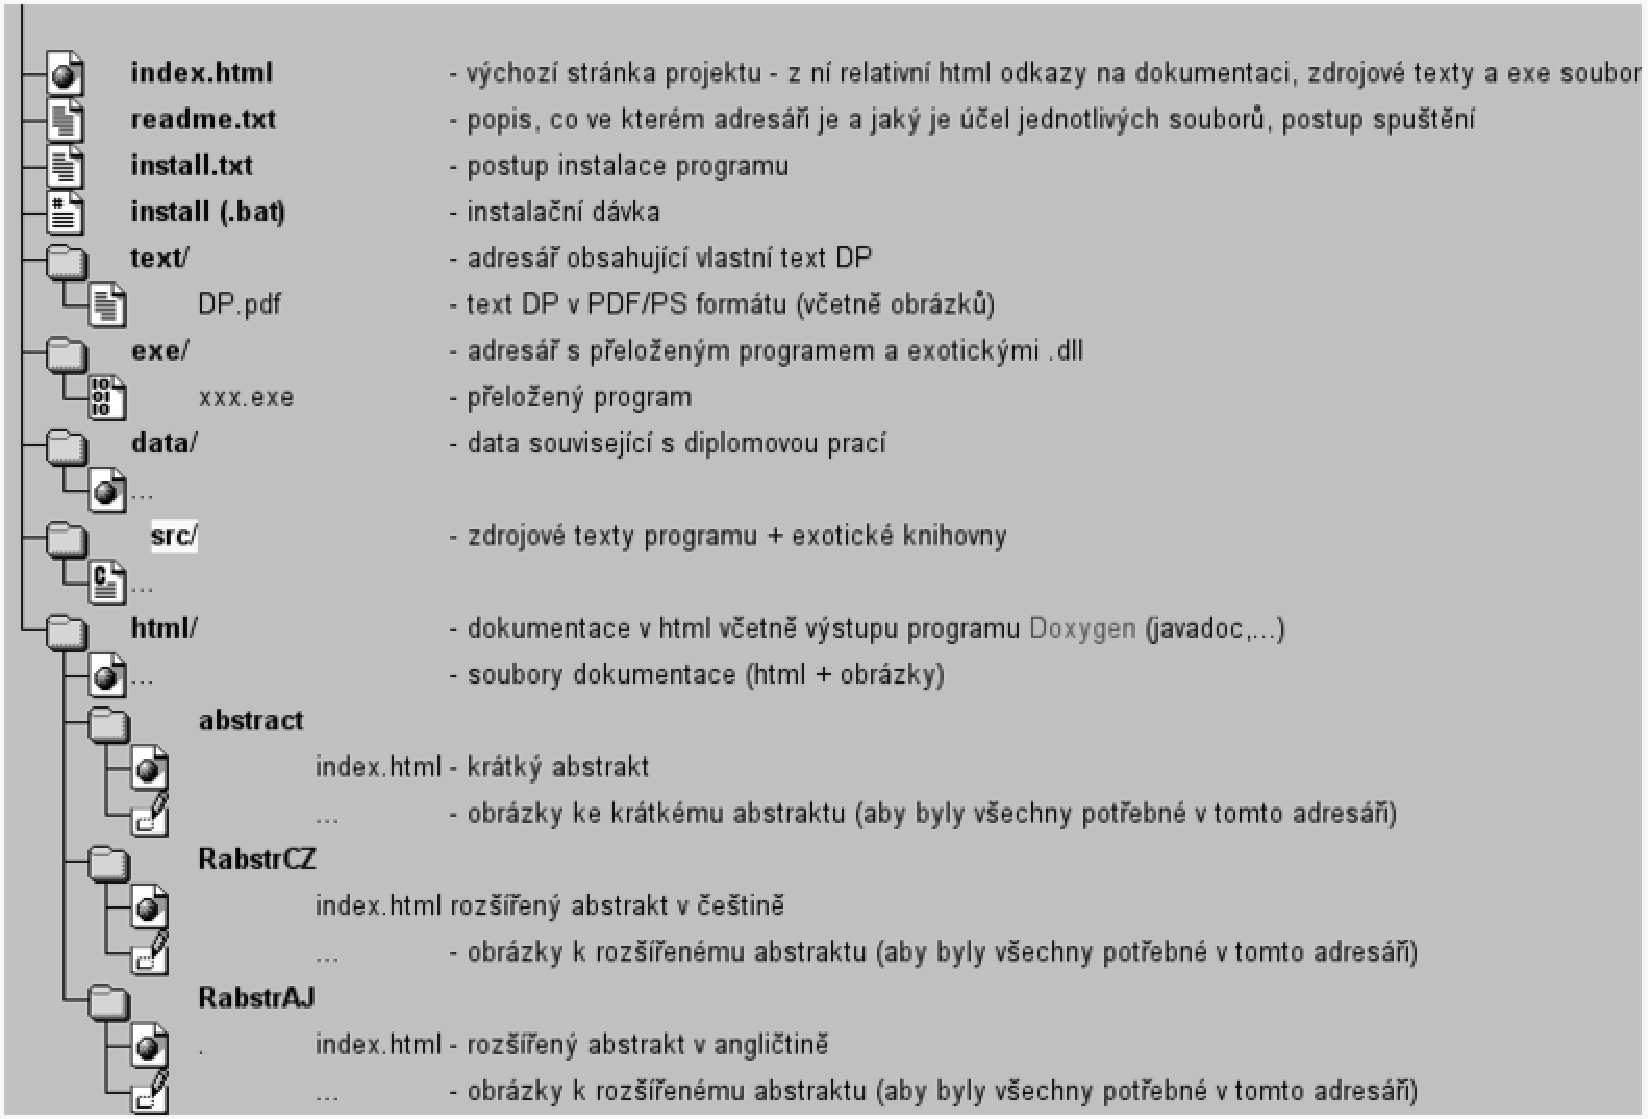
\includegraphics[width=14cm]{figures/seznamcd}
\caption{Seznam přiloženého CD --- příklad}
\label{fig:seznamcd}
\end{center}
\end{figure}

\end{document}
